\documentclass{template/abschlussarbeit}

%%%%%%%%%%%%%%%%%%%%%%%%%%%%%%%%%%%%%%%%%%%%%%%%%%%%%%%%%%%%
% Allgemeine Variablen fuer die Abschlussarbeit (mit eigenen
% Angaben ausfuellen!)
%%%%%%%%%%%%%%%%%%%%%%%%%%%%%%%%%%%%%%%%%%%%%%%%%%%%%%%%%%%%

\AutorVorname{Johannes}
\AutorNachname{Thiel}
\AutorGeburtsort{Solingen}
\AbschlussarbeitTitel{Meine Abschlussarbeit}
% Bachelorarbeit, Projektarbeit, Masterarbeit
\AbschlussarbeitTyp{Masterarbeit}
% keywords durch , getrennt
\AbschlussarbeitKeywords{Distributed Systems, Big Data, Cloud}
\Ort{Düsseldorf}
\Datum{19. November 2015}
\Erstgutachter{Prof. Dr. Michael Schöttner}
\Zweitgutachter{Prof. Dr. Stefan Conrad}
\Betreuer{Msc. Bernd Mustermann}

% Hier den vollstaendigen Dateinamen der bibtex Datei angeben
% Falls diese in einem Unterordner liegt, so ist dieser relativ
% zu dieser Datei (document.tex) anzugeben.
\LiteraturBibtexDatei{librarys}

% Der Anhang (falls vorhanden) wird hier genauso wie diese
% Bibtex-Datei angegeben (jedoch ohne .tex-Endung!)
\AnhangDatei{chap/anhang}

%%%%%%%%%%%%%%%%%%%%%%%%%%%%%%%%%%%%%%%%%%%%%%%%%%%%%%%%%%%%
% Optionen/Schalter um bestimmte Abschnitte an-/auszuschalten
% WICHTIG: Nicht genutzte/leere Abschnitte vor der Abgabe/
% dem finalen Druck abschalten durch auskommentieren.
% Gleiches gilt fuer die Todo Liste, welche nicht in die 
% finale Version gehoert.
%%%%%%%%%%%%%%%%%%%%%%%%%%%%%%%%%%%%%%%%%%%%%%%%%%%%%%%%%%%%

\Titelblatt
\TodoListe
\Inhaltsverzeichnis
\Abbildungsverzeichnis
\Tabellenverzeichnis
\Algorithmenverzeichnis
\Anhang
\Erklaerung

%%%%%%%%%%%%%%%%%%%%%%%%%%%%%%%%%%%%%%%%%%%%%%%%%%%%%%%%%%%%

\begin{document}
\begin{abschlussarbeit}

%%%%%%%%%%%%%%%%%%%%%%%%%%%%%%%%%%%%

% Hier werden die einzelnen Kapitel aufgelistet (Reihenfolge!)
% Die vorgegebenen Kapitel dienen als Hilfestellung waehrend der Arbeit
% und sind mit der Fertigstellung des finalen Dokuments zu entfernen!
\chapter{Grundlagen}

\section{Graphen}


Im Allgemeinen kann ein Graph durch $G = (V, E)$ dargestellt werden, wobei $V$ eine Menge an Knoten und $E$ eine Menge an Kanten ist. Die Kanten sind jeweils ein geordnetes Knotenpaar $(u, v) \subseteq V \times V$.

\subsection{Dichte}
\label{dichte}

Die Dichte eines Graphen gibt das Verhältnis zwischen der Anzahl an Kanten und der potentiell möglichen Anzahl an Kanten an \cite{diestel2010graphentheorie}.
Sie lässt sich bestimmen mit:

\[ d(G) =  \frac{2|{E}|}{|V|(|V| - 1)}    \]


\subsection{Knotengrad}
\label{knotengrad}

In einem gerichteten Graphen besitzt jeder Knoten einen Ausgang- und Eingangsgrad. Dies ist jeweils die Anzahl an Kanten, die bei dem Knoten starten bzw. bei ihm enden \cite{diestel2010graphentheorie}.
Der Ausgangsgrad für einen Knoten $v$ im Graph $G$ wird mit $d^{+}_{G}(v)$ und den Eingangsgrad mit $d^{-}_{G}(v)$ bezeichnet.



\subsection{Multi Layer Graphen}

Im Folgenden werden Multi Layer Graphen betrachtet. Diese Graphen haben neben Knoten und Kanten auch eine Menge an Ebenen. Dabei kann, je nach Art des Graphen, der gleiche Knoten in verschiedene Ebenen vorhanden sein oder auch Verbindungen zwischen den Knoten in verschiedenen Ebenen bestehen.
Welche Bedeutung den Ebenen zukommt, hängt vom Graphen und dem Anwendungsfall der Daten ab. Multi Layer Graphen können genutzt werden, um Netzwerke in unterschiedlichen Themengebieten abzubilden, z.B. soziale Netzwerke, Transport oder Biologie.

Multi Layer Graphen können, abhängig von ihren Verbindungen, in verschiedene Kategorien eingeteilt werden. Die verschiedenen Kategorien sind in Abbildung \ref{network_types} dargestellt. 

\begin{figure}
  \centering
  \begin{subfigure}[b]{1.0\textwidth}
    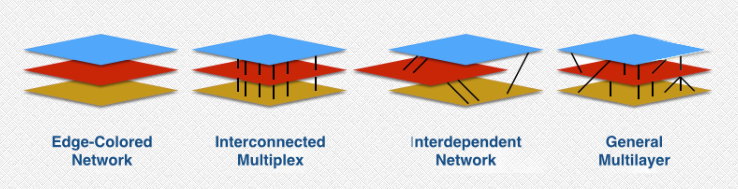
\includegraphics[width=1.0\linewidth]{img/network_types.png}
  \end{subfigure}
  \caption{Multi Layer Netzwerkarten}
  \label{network_types}
\end{figure}

\subsubsection{Edge Colored Network}

In Edge Colored Networks gibt es nur Kanten zwischen Knoten im gleichen Layer. Dabei sind die Kanten jeweils mit einem Label versehen das kennzeichnet, zu welchem Layer sie gehören.


\subsubsection{Interconnected Multiplex}

In Multiplex Netzwerken gibt es hauptsächlich Kanten zwischen Knoten, die sich im gleichen Layer befinden. Die einzigen Kanten, die es zwischen verschiedenen Layern gibt, verbinden jeweils den gleichen Knoten in dem anderen Layer. 

\subsubsection{Inderdependet Network}

In Inderdependet Networks gibt es keine Knoten, die in mehr als einem Layer vorkommen. Kanten können Knoten innerhalb eines Layers, aber auch zwischen zwei Layern verbinden.

\subsubsection{Generelle Multi Layer}
In einem Generellen Multi Layer Graph gibt es keine Restriktion, wie die Knoten der verschiedene Ebenen miteinander verbunden sein können. Es kann sowohl Verbindungen zwischen dem gleichen Knoten in verschiedenen Ebenen geben, als auch Verbindungen zu Knoten in anderen Ebenen.


Ein genereller Multi Layer Graph kann formal als ein gerichteter Multigraph\cite{multiLayerMath} $G = (\Sigma_{V}, \Sigma_{E}, V, E, s, t, l_{V}, l_{E})$, dessen Knoten und Kanten ein Label besitzen, definiert werden, wo

\begin{itemize}
  \item V die Menge an Knoten und E die Menge an Kanten ist
  \item $\Sigma_{V}$ und $\Sigma_{E}$ die Alphabete sind, die als Label für Knoten und Kanten dienen
  \item $s: E \rightarrow V$ und $t: E \rightarrow V$ zwei Zuordnungen sind, die angeben, von welchem Knoten eine Kante ausgeht und zu welchem sie führt
  \item $l_{V}: V \rightarrow \Sigma_{V}$ und $l_{E}: V \rightarrow \Sigma_{E}$ zwei Zuordnungen sind, die den Knoten und Kanten ihre Labels zuweisen
\end{itemize}

Da mit den Generellen Multilayer Graphen auch alle anderen Arten von MultiLayer Graphen dargestellt werden können, werden im Folgendem nur noch Generelle Multigraphen betrachtet.


\section{Page Rank}

Page Rank wurde von Larry Page, Sergey Brin, R. Motwani und T. Winograd in der Arbeit The PageRank Citation Ranking:
Bringing Order to the Web\cite{Page98thepagerank} vorgestellt. Sie beschreiben, wie PageRank genutzt werden kann um die Wichtigkeit von Internetseiten zu bewerten.

Neben Internetseiten kann PageRank aber auch auf andere Graphen angewandt werden.
PageRank bewertet Knoten in einem Graphen anhand von ihren Kanten. Knoten erhalten eine hohe Bewertung, wenn sie viele eingehenden Kanten besitzen. Auch die Bewertung der Knoten von denen die eingehenden Kanten ausgehen wirkt sich auf die Bewertung aus.

Da, die Daten verteilt auf mehren Servern liegen und keine globale Sicht existiert wird die iterative Variant von PageRank betrachtet.
Bei dieser verteilt jeder Knoten in jeder Iteration seinen eigenen PageRank Wert gleichmäßig auf alle Knoten zu denen er ausgehende Kanten besitzt. 


Sei $ PR(p_{i}; t)$ der PageRank Wert des Knoten $p_{i}$ zu dem Iterationsschrit $t$ und die gesamte Zahl aller Knoten $N$.
Zudem sei $M(p_{i})$ die Knoten die eine ausgehende Kante zu $p_{i}$ haben und $L(p_{i})$ die Anzahl an ausgehenden Kanten von Knoten $p_{i}$.
Jeder Knoten startet mit einem PageRank Wert von

\[  PR(p_{i}; 0) = \frac{1}{N}   \]

Bei jedem Iterationsschrit wird für jeden Knoten ein neuer Wert mit folgender Formel berechnet:

\[ PR(p_{i}; t+1) = \frac{1 - d}{N} + d \sum_{p_{j} \in M(p_{i})} \frac{PR(p_{j}; t)}{L(p_{j})} \]


Dabei ist $d$ ein Dämpfungsfaktor, der verhindert das einzelne Knoten, die keine ausgehenden Knoten besitzen die einzigen sind die keinen Wert von 0 am Ende haben.

Als Abbruchbedingung für die Iterationen können eine feste Anzahl an Iterationsschritten gewählt werden. Alternativ kann auch ein Grenzwert $\epsilon$ festgelegt werden und der Algorithmus bricht ab sobald die Veränderung aller Werte unter $\epsilon$ liegt.


\section{HITS}

Hubs and Authorities (HITS) wurde von John M. Kleinberg in Authoritative Sources in a Hyperlinked Environment \footnote{\cite{Kleinberg98authoritativesources}} vorgestellt.

Dabei werden in einem Netzwerk aus aufeinander verweisenden Doukumenten beurteilt. Beispiele für solche Netzwerke sind Internetseiten die aufeinander
verlinken oder Wissenschaftliche Veröffentlichung die einander refenzieren. Ein Hub sind Dokumente die auf viele gute Quellen verweisen, während
Authorities Doukumente sind die gute Quellen sind und auf welche oft verwiesen wird. Der Algorithmus läuft ähnlich zum PageRank-Algorithmus ab 
jedoch wird nicht nur ein einzelner Werte für jeden Knoten bestimmt sonder jeweils ein Hub und Authority Werte pro Knoten. Umso höher der Wert umso
ein besser Hub oder Authority ist ein Knoten.

Für einen gerichteten Graphen $G = (V, E)$ weisen wir jedem Knoten $v \in V$ einen Authority $x_{v}$ und Hub $y_{v}$ Wert zu.

HITS ist ein iterativer Algorithmus der für jeden Knoten eines Graphen jeweils einen Hub und einen Authority Wert bestimmt. Hierfür 
werden jeweils die Hub oder Authority Werte der benachbarten Knoten genutzt. Damit die Authority und Hub Werte sich nicht gegen
unendlich aufschaukeln werden sie in jeder Iterationen so normalisiert das die Summe der Quadrate 1 ergibt:
$ \sum x_{i}^{2} = 1 $ und $ \sum y_{i}^{2} = 1$.
Die Werte für jeden Knoten konvergieren im laufe der Iterationen.

HITS aktualisiert zuerst die Authority Werte der Knoten und danach die Hub Werte.

Authority Update:

Für jeden Knoten $ v \in V $ wird der neue Authority Wert aus der Summe der Hub Werte der eingehenden Kanten gebildet.

\[ x_{p} = \sum_{q; (q, p) \in E} y_{q} \]


Danach werden alle Authority Werte wie oben beschrieben normalisiert:

$ x_{p} =  \frac{x_{p}}{\sum x_{q}^{2}} $

Hub Update:

Genauso


Um den Algorithmus konvergieren zu lassen wähle ein $ \epsilon $ und prüfe nach jeder Iteration ob die gesammte Änderung der Authority
und Hub Werte kleiner als das $ \epsilon $ ist. Ist dies nicht der Fall werden weitere Iterationen durchgeführt.


\section{Andere Multilayer Graph Systeme}

Im Folgendem werden verschiedene andere Systeme betrachtet, mit denen Multilayer Graphen analysiert werden können.

\subsection{MuxViz}

Das Analysetool MuxViz wurde von De Domenico, M. und Porter, M. A. und Arenas, A. in ihrer Arbeit ''MuxViz: a tool for multilayer analysis and visualization of networks vorgestellt'' \cite{De_Domenico_2014}.
MuxViz ist ein open-source Projekt, welches es ermöglicht Multilayer Graphen mit verschiedenen Algorithmen zu analysieren und visualisieren. Es nutzt für die Berechnungen R sowie GNU Octave und bietet mit einem modularen Aufbau die Möglichkeit, das Nutzer eigene Funktionalität hinzufügen.


MuxViz bietet eine grafische Nutzeroberfläche, welche genutzt werden kann, um Graphen zu laden, Algorithmen auszuführen und Graphen sowie Ergebnisse zu visualisieren. Die Benutzeroberfläche ist Webbasiert, was ermöglicht, dass die tatsächlichen Berechnung entweder lokal oder auf einem entfernten Server durchgeführt werden.
Dabei gibt es eine große Auswahl an Algorithmen und Statistiken, die auf den Graphen angewandt werden können.


%\begin{figure}
%  \centering
%  \begin{subfigure}[b]{1.0\textwidth}
%    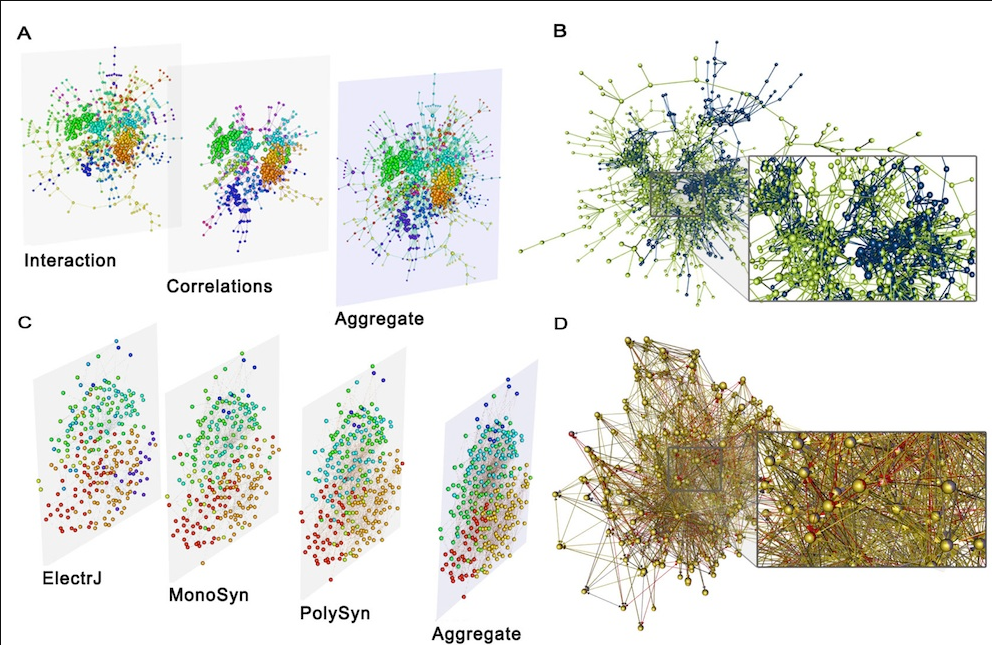
\includegraphics[width=1.0\linewidth]{img/muxViz.png}
%  \end{subfigure}
%  \caption{muxViz}
%  \label{muxVizSample}
%\end{figure}

\subsection{Multilayer Networks Library for Python}

Die Multilayer Networks Library for Python (Pymnet) wurde von Mikko Kivelä 2015 veröffentlicht. 
Die in Python geschriebene Bibliothek ermöglicht es mit Multilayer Netzwerke in Python zu arbeiten. Sie unterstützt das Laden und Manipulieren von Multilayer Netzwerken und bietet eine Reihe an Algorithmen zur Analyse der Netzwerke.
Zudem können Netzwerke mithilfe von Matplotlib und D3 visualisiert werden.


\section{Graph Engine}

Graph Engine ist ein verteiltes in-Memory Datenverarbeitungssystem, welches von Microsoft Research Asia 
entwickelt wurde \cite{graphEngine}. Der Quellcode von Graph Engine ist quelloffen auf Github verfügbar und in C\# geschrieben.

Es bietet einen verteilten Key-Value Speicher, in dem Daten gespeichert und verarbeitet werden können. Dabei ist Graph Engine sehr flexibel darin, wie die Daten gespeichert werden. Der Anwender muss selbst
Schemata für die zu speichernden Daten erstellen. Dazu bietet Graph Engine die Möglichkeit, die Kommunikation unter den verschiedenen Servern mit selbst erstellten Protokollen zu koordinieren. Im Folgenden werden die verschiedenen Komponenten von Graph Engine besprochen.

\subsection{Memory Cloud}
\label{memoryCloud}

Im Kern von Graph Engine steht die sogenannte Memory Cloud. Diese stellt einen verteilten Key-Value Speicher dar, der im Arbeitsspeicher der Maschinen
liegt, um einen schnellen Zugriff zu gewährleisten.

Graph Engine verwaltet sogenannte Memory Trunks, in denen die Key-Value Paare gespeichert werden. Jeder der Trunks ist auf einer Maschine gespeichert.
In der Regel gibt es mehr Trunks als Maschinen, sodass eine Maschine mehrere Trunks hält. Durch die Aufteilung in mehrere Trunks kann parallel auf Daten aus verschiedenen Trunks zugegriffen
werden, ohne das ein weiterer Lock-Mechanismus benötigt wird. Die Größe der Trunks kann manuell gewählt werden, liegt aber bei den Standardeinstellungen bei 2GB.
Um zu gewährleisten, dass die Daten wiederhergestellt werden können, werden die Memory Trunks in dem verteilten Dateisystem Trinity File System (TFS) gespeichert. Das Design von TFS ist ähnlich zu Googles HDFS.

Als Schlüssel für die Werte werden 64-Bit Werte verwendet.
Die Werte selbst sind beliebig große Datenblobs, die direkt im Arbeitsspeicher der Maschinen verwaltet werden.


Um einen Wert anhand des Schlüssels zu finden, werden zwei Schritte durchgeführt. Zuerst wird die Maschine gefunden, die für den jeweiligen Schlüssel
verantwortlich ist. Danach wird der Schlüssel in den Memory Trunks dieser Maschine gefunden.

Im ersten Schritt wird der Schlüssel auf einen p-Bit Wert gehasht, um ein  $ i \in [0, 2^{p} - 1] $ zu erhalten. Der Schlüssel liegt demnach in
Memory Trunk $ i $. Jede Maschine besitzt eine Adressierungstabelle, die festhält, welcher Trunk auf welcher Maschine liegt.

Auf dieser Maschine muss nun der Schlüssel gefunden werden. Dafür besitzt jeder Memory Trunk eine Hashtabelle, die zu jedem Schlüssel
ein Offset und die Größe des Wertes im Speicher angibt.

\subsection{Graph Model}

Graph Engine bietet ein flexibles Model, mit dem die Graphdaten modelliert werden können. Es gibt keine festgelegte Struktur und es ist den Entwicklern
überlassen, Schemata für die Daten festzulegen. Hierbei hat man die Möglichkeit das Graphmodell genau an das zu lösende Problem anzupassen.
Dies bietet die Chance Optimierungen zu finden und gibt eine sehr feine Kontrolle über die gespeicherten Daten.

\subsubsection{Trinity Specification Language (TSL)}

Um das Datenmodell zu definieren, benutzt Graph Engine eine eigene Sprache, die Trinity Specification Language (TSL). Mit dieser werden sowohl die Schemas
für Daten, als auch Server Protokolle und Schnittstellen erstellt. 

TSL bietet die Möglichkeit Zellen zu definieren, welche im Betrieb als Werte im Key-Value Speicher abgelegt werden können.
Zellen können Grunddatentypen wie int, float, string etc. sowie Listen von Werten speichern. Um komplexere Werte darzustellen, können auch in TSL erstellte structs verwendet werden.
Mit diesen Möglichkeiten lassen sich sehr viele Datenstrukturen in TSL modellieren. 

Ein Beispiel für einen simplen Graphen ist in  \ref{lst:tsl} dargestellt. In diesem Beispielgraph hat jeder Knoten 
einen Wert und eine Liste an Kanten. Die Kanten selbst haben ein Gewicht sowie einen Verweis auf die ID des Knoten, auf den sie zeigen.

\begin{lstlisting}[language=c,label={lst:tsl}, caption={Beispiel für eine in TSL definierte Graphenstruktur}]
struct Edge {
  float Weight;
  long Link;
}

cell struct GraphNode {
  int Value;
  List<Edge> Edges;
}
\end{lstlisting}



Graph Engine hat einen eigenen Compiler für TSl, der die TSl Dateien in C\# Quellcode umwandelt. So werden aus den Definitionen Schnittstellen
generiert, um die entsprechenden Zellen in Graph Engine zu erstellen, zu verändern oder zu löschen. 

\subsection{Computation Engine}

Um Berechnungen durchzuführen, besteht ein Graph Engine Cluster aus drei verschiedenen Komponenten, die unterschiedliche Aufgaben übernehmen.


\subsubsection{Server}

Die Server in einem Graph Engine Cluster haben zwei Aufgaben: Zum einem speichern sie die Memory Trunks in ihrem Arbeitsspeicher, 
zum anderen führen sie Berechnungen auf den gespeicherten Daten durch.
Um diese Berechnungen durchzuführen, werden in der Regel Nachrichten mit anderen Graph Engine Komponenten ausgetauscht. Insbesondere die Kommunikation zwischen den Servern
selbst ist oft notwendig, da jeder Server nur eine Sicht auf seine lokal gespeicherten Daten hat.

\subsubsection{Proxy}

Proxies speichern selber keine Daten, können aber Nachrichten austauschen und Berechnungen durchführen. Sie können als 
Bindeglied zwischen Client und Server genutzt werden. So können sie z.B. von Clients geschickte Anfragen auf die Server aufteilen und deren
Berechnungen koordinieren oder die einzelne Ergebnisse aggregieren. Insbesondere in aufwändigeren Algorithmen kann eine Proxy 
den Ablauf kontrollieren und Entscheidungen wie Abbruchsbedingungen prüfen.

\subsubsection{Client}

Clients laufen auf der Maschine des Benutzers, der mit dem Graph Engine Cluster interagieren will. Clients senden Anfragen an die Server oder Proxies und
erhalten die entsprechenden Ergebnisse zurück. Sie halten keine Daten und führen in der Regel auch keine Berechnungen durch, womit es keine großen Hardwareanforderungen
an die Maschine gibt, auf der ein Client läuft.

\subsubsection{Protokolle}

Server, Proxies und Clients kommunizieren über Nachrichten, die sie einander schicken. Graph Engine unterstützt hierbei drei verschiedene Arten von Protokollen.


Synchrone Protokolle sind ähnlich zu synchronen Funktionaufrufen, die auf einer anderen Maschinen stattfinden. Sie blockieren die weitere Ausführung, bis
eine Antwort erhalten wurde. Ein Synchrones Protokoll kann sowohl in der Anfrage, als auch in der Antwort Daten mitsenden. So kann beispielsweise die Liste von
relevanten Schlüsseln übergeben werden und mit deren Gesamtsumme der Werte geantwortet werden.


Asynchrone Protokolle blockieren die Ausführung des Absenders nicht. Der Empfänger antwortet beim erhalten der Anfrage sofort mit der Bestätigung, dass diese erhalten wurde.
In einem Synchronen Protokoll können lediglich in der Anfrage Werte mitgegeben werden.
Der Empfänger startet einen Thread, der die Anfrage abarbeitet. Der Absender erfährt nicht, wann die Anfrage vollständig bearbeitet wurde.


HTTP Protokolle bieten Clients die Möglichkeit eine RESTful Version der Synchronen Protokolle über HTTP zu nutzen. Graph Engine erstellt automatisch die Endpunkte, an denen
auf Anfragen gewartet wird. So wird z.B. für ein Protokoll \verb|MyHTTProtocol| am Endpunkt

\verb|http://example.com/MyHttpProtocol| gewartet. Die Anfrage und
Antwort werden jeweils in JSON Strukturen übergeben. HTTP Protokolle werden nicht für Server zu Server Kommunikation genutzt, da sie deutlich weniger effizient sind als die
Synchronen und Asynchronen Protokolle.

\subsubsection{TSL}

Die Kommunikationschemata von Servern und Proxies werden in TSL definiert. In \ref{lst:ping} ist ein Beispiel für einen Server, der ein Synchrones Ping Protokoll unterstützt, dargestellt.

\begin{lstlisting}[language=c,label={lst:ping}, caption={In TSL definiertes Ping Protokoll}]
struct PingMessage {
  string Content;
}

protocol SynEchoPing {
  Type: Syn;
  Request: PingMessage;
  Response: PingMessage;
}


server PingServer {
  protocol SynEchoPing;
}
\end{lstlisting}

Wie schon bei den Zellen werden die Server und Protokolldefinitionen von dem TSL Compiler in C\# Code übersetzt. Für Server und Proxy
Definitionen werden abstrakte Klassen erstellt, in denen jeweils Methoden für die benötigten Protokolle implementiert werden müssen.
Es werden zudem Methoden generiert, um die definierten Anfragen an den Server oder die Proxy zu erstellen und diese zu senden.


\subsection{Datenzugriff}
\label{geAccessor}

Die Daten der Zellen liegen im Arbeitsspeicher der Maschinen als Datenblobs. Um auf diese komfortabel zuzugreifen, können die Daten in ein C\# Objekt
serialisiert werden; das ist jedoch sehr langsam.
Schnelleren Zugriff hat man, indem man die Daten direkt im RAM manipuliert. Das ist jedoch deutlich schwieriger, da man das Speicherlayout der jeweiligen Daten
kennen und entsprechende Zeiger-Arithmetik betreiben muss. Graph Engine löst diesen Konflikt, indem es aus der TSL Zellendefinition eine Zugriffklasse erzeugt.
Diese übersetzt die Lese- und Schreibzugriffe auf die Werte der Zelle auf die entsprechenden Operationen im Arbeitsspeicher. So lässt sich mit der Zugriffklasse sowohl
komfortabel, als auch effizient arbeiten.

\begin{lstlisting}[language=c, caption={Bearbeitung einer Zelle mithilfe der Zugriffklasse}]
  using (var node = Global.LocalStorage.UseNode(cellId, accessOptions)) {
    int value = node.Value;
    node.Value = 5;
  }
\end{lstlisting}


\chapter{Hauptteil}

\section{Graph Engine}

Da Graph Engine eine wichtige Rolle in dem MultiLayer Graph System spielt, werden im Folgenden einige Dinge betrachtet, die wichtig für die Verwendung von Graph Engine sind.
Dies ist insbesondere interessant, da die aktuelle Version 2 von GraphEngine sich zurzeit noch in Entwicklung befindet und dadurch die Verwendung durch fehlende Dokumentation erschwert wird.


\subsection{Einrichtung}

Graph Engine wurde in C\# entwickelt und verwendet den dafür verbreiteten Paket-Manager NuGet, mit dem Pakete verwaltet werden können.
Die aktuellste Version von dem GraphEngine.Core Paket auf NuGet ist 1.0.8467 vom 	19.08.2016 \cite{geVersion}. Da in dieser Arbeit die Version 2.0.9912 verwendet wird, ist es nötig, dass GraphEngine.Core Paket selber vom Quellcode aus zu bauen.
Der Quellcode ist auf Github in dem Repository https://github.com/microsoft/GraphEngine zu finden. Dabei ist auch die Anleitung zum kompilieren des Pakets.


\subsubsection{Konfigurationsdatei}

Graph Engine benutzt eine .xml Konfigurationsdatei, um das Cluster aus Proxy und Servern zu definieren.
In der Datei können zudem weitere Einstellungen, wie Dateipfade oder Logging, für die Server gemacht werden (siehe \ref{lst:config}).

\begin{lstlisting}[language=xml, label={lst:config}, caption={Beispiel Konfigurationsdatei für ein Cluster mit einer Proxy und zwei Servern}]
<Trinity ConfigVersion="2.0">
  <Cluster>
    <Proxy Endpoint="node52:8133" LogDirectory="D:\log-dir" LoggingLevel="Info" />  
    <Server Endpoint="node55:8133" />
    <Server Endpoint="node63:8133" />
  </Cluster>
</Trinity>
\end{lstlisting}


\subsection{Datenzugriff}
\label{datenzugriff}

Graph Engine bietet mehrere Arten auf die Daten von Zellen zuzugreifen. Dabei ist es wichtig zu verstehen, wie die verschiedenen Arten funktionieren und wie deren Performance ist.

Die erste Möglichkeit ist auf Zellen von entfernten Maschinen zuzugreifen. Dabei werden die Funktionen der \verb|Global.CloudStorage| verwendet. Dies ist die langsamste Art , da für jeden Zellenzugriff eine Netzwerknachricht an die entfernte Maschine geschickt werden muss.

Dazu gibt es zwei weitere Möglichkeiten auf lokale Zellen mittels \verb|Global.LocalStorage| zuzugreifen. Die erste ist \verb|LoadCell()|. Diese Methode lädt die Daten einer Zelle aus dem von GE verwalteten Arbeitsspeicher in ein Objekt des C\# Heaps.
Dabei wird jedes Mal ein neues Objekt erzeugt und die Werte in dieses kopiert. Hiermit kann nur auf die Daten der Zelle zugegriffen, diese aber nicht verändert werden.

Die andere Methode ist der direkte Zugriff über \verb|UseCell()|. Dabei wird direkt auf die im Arbeitsspeicher vorhandene Zelle zugegriffen, ohne das diese kopiert werden muss (siehe \ref{geAccessor}). Dazu können so auch die Werte der Zelle direkt verändert werden. Diese Methode ist damit von der Performance her die beste Art auf Zellen zuzugreifen und sollte, wenn möglich, immer verwendet werden.



\subsection{Schwierigkeiten}

Da sich die Version 2 von GraphEngine noch in Entwicklung befindet, gibt es einige Schwierigkeiten, die bei der Entwicklung von Anwendungen mit Graph Engine entstehen.

Hauptsächlich ist hierbei die kaum vorhandene Dokumentation für Version 2 problematisch. Viele Änderungen zwischen den beiden Versionen sind nicht dokumentiert. So wurden zum Beispiel
das Attribut jeder Zelle, welches die ID der Zelle beinhaltete, von \verb|cell.CellID| zu \verb|cell.CellId| umbenannt. Auch wurde die Bezeichnung für entfernte Server von \verb|Server| zu \verb|Partition| geändert.
Solche Änderungen machen das Entwickeln von Anwendungen mit GraphEngine zeitaufwändig, da immer wieder im Quellcode nachgeschaut werden muss wie bestimmte Dinge heißen. 

Dazu sind viele Funktionen auch wenig oder gar nicht dokumentiert. So zum Beispiel die Funktion \verb|Global.CloudStorage.BarrierSync(int)|, welche es erlaubt die Server an einer Barriere warten zu lassen, bis alle diese erreicht haben.
Dies macht es schwierig alle Möglichkeiten von GraphEngine auszunutzen und erfordert regelmäßiges Nachforschen im Quellcode, ob gewisse Funktionen vorhanden sind und was diese im Detail machen.

Zudem sind alle Beispielanwendungen, die es im GraphEngine Repository gibt, noch auf Version 1 und einige dadurch nicht kompatibel mit der neueren Version.





\section{Architektur}

Das MultiLayer Graph System setzt sich aus mehren Komponenten zusammen, die miteinander arbeiten, um die gewünschten Anforderungen zu gewährleisten.
Dabei wird GE genutzt, um die Graph Daten effizent im Arbeitsspeicher der Server zu verwalten und die Kommunikation der einzelnen Komponenten zu steuern.  Das TSL-Model und eine geteilte Bibliothek bieten die Basis für die
anderen Komponenten.

In der Architektur ist der Client für das Senden von Anfragen, sowie das Ausführen eines Algorithmus oder das Laden eines Graphen an die Proxy zuständig.
Die Proxy verarbeitet die Anfrage und koordiniert ggf. die Berechnungen der Server. Die Server kommunizieren, falls nötig für ihre Berechnungen untereinander, um Daten über entfernte Knoten anzufragen oder zu senden. Sobald die Anfrage fertig bearbeitet ist, schickt die Proxy eine Antwort mit den enstprechnden Ergebnissen an den Client.
Eine Darstellung dieser Arbeitsweise ist in Abbildung \ref{architektur} dargestellt.

\begin{figure}
  \centering
  \begin{subfigure}[b]{1.0\textwidth}i
    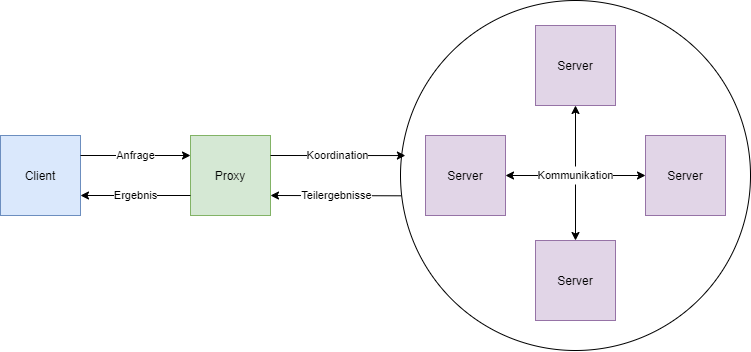
\includegraphics[width=1.0\linewidth]{img/Architektur-Cluster.png}
  \end{subfigure}
  \caption{Aufbau des Multilayer Clusters}
  \label{architektur}
\end{figure}



\subsection{Model}

Das TSL Model dient als Basis für den Rest der Anwendung. Es wird definiert, wie Knoten gespeichert werden und wie Client, Server und Proxy miteinander
kommunizieren können. Die einzelnen Komponenten müssen die von GE automatisch generierten Klassen implementiernen.


Es wird die grundlegende Graphenstruktur definiert, die genutzt wird, um Multilayer Graphen darzustellen. Knoten speichern hierbei jeweils ihre ID, zu welchem Layer sie gehören
und ihre Liste an ausgehenden Kanten. Dazu kommen Daten, die gebraucht werden, um Algorithmen auszuführen. Die können z.B. der aktuelle PageRank Wert des Knoten sein.


\subsection{Lib}

Die geteilte Bibliothek besteht aus zwei Komponenten. Sie enthält den von TSl generierten Code und macht es so dem Client/Proxy/Server möglich darauf zuzugreifen. Der generierte Code enthält auch die abstraken Klassen für Proxy und Server. Diese werden in den enstprechnden Komponenten implementiert. 

Außerdem enthält sie eine Sammlung aus Funktionen, die alle Projekte nutzen können. Insbesondere besitzt sie ein Interface, um mit dem Graphen zu interagieren und z.B. neue Knoten anzulegen oder einem Knoten neue Kanten hinzuzufügen.
Dazu kommt die Funktionalität, Ergebnisse von Algorithmen ausgeben zu lassen, da dies sowohl auf dem Client, als auch der Proxy möglich ist.


\subsection{Client}

Der Client stellt die Schnittstelle zwischen dem Anwender und dem Multilayer System dar. Der Client kann Anweisungen des Anwenders auf zwei Arten empfangen.
Zum einem wird ein Kommandozeilen Interface bereitgestellt, mit dem der Anwender interagieren kann. Zum anderen kann dem Client eine batch Datei mit Anweisungen übergeben werden,
welche nacheinander ausgeführt werden.
Hierbei besteht auch die Möglichkeit zwischen dem Interaktiven und dem Batch Modus zu wechseln.

Die Anweisungen werden interpretiert und in Anfragen an die Proxy übersetzt, welche die Anfragen dann abarbeitet.

\subsection{Proxy}

Die Proxy dient als Bindeglied zwischen dem Client und den Servern. Sie nimmt Anfragen vom Client an und sorgt dafür, dass diese ausgeführt werden.
Dabei koordiniert sie die Ausführung der verschiedenen Algorithmen und sendet die nötigen Anfragen an die Server. Wenn es nötig ist, kann gewartet werden,
bis alle Server die Anfrage abgearbeitet haben. Die Server können dabei auch ein Ergebnis zurücksenden, welches die Proxy weiter verwenden kann. Ein häufiger Fall
ist hierbei, dass die Ergbenisse der einzelnen Server aggregiert werden.


Abhänging von der Client Anfrage ist die Proxy auch für das Messen der Laufzeit und das Bilden der Ergebnisse verantwortlich. Die Ergebnisse können im gewünschten Format entweder direkt auf der Proxy ausgegeben
oder zurück an den Client gesendet werden.

\subsection{Server}

Die Server erfüllen zwei Aufgaben. Sie verwalten die Graph Daten in GE und warten darauf, dass sie Anweisungen von der Proxy bekommen und führen auf ihre Anweisung Berechnungen durch. Bei diesen Berechnungen kümmert sich jeder Server 
um die eigenen lokal gespeicherten Knoten. Die Serven können aber auch miteinander kommunizieren, wenn sie die Daten entfernter Knoten benötigen oder die Daten entfernter Knoten
aktualisieren müssen.
Ist ein Server mit einer angeforderten Aufgabe fertig, kann er dies der Proxy melden. Dabei kann, falls nötig, auch ein Ergebnis mitgesendet werden.





\section{Implementierung}

Im folgendem wird auf die Implementierungsdetails der einzelnen Komponenten eingegangen. Hierbei wird der grundlegende Aufbau der Komponenten erklärt.
Zudem wird auf einige Optimierungen und Designentscheidungen eingegangen.


\subsection{Model}



Um Multilayer Graphen in GE abzubilden wird pro Knoten und Layer eine Zelle erstellt. Die Zellen speichern hierbei ihre ID ihren Layer, eine Liste der ausgehenden Kanten und Daten die für die ALgorithmen notwendig sind.
Die Kanten müssen dabei speichern auf welche ID in welchem Layer sie zeigen.

\begin{lstlisting}{language=c,label={lst:tslModel}}
struct Edge {
  long StartId;
  int StartLayer;
  long DestinationId;
  int DestinationLayer;
  float Weight;
}

// We create a cell for each layer a node is on
cell struct Node {
  long Id;
  int Layer;
  PageRankData PageRankData;
  HITSData HITSData;
  DegreeData DegreeData;
  List<Edge> Edges;
}
\end{lstlisting}

Die Proxy wird mit allen unterstützen Protokollen definiert. 

Die Proxy muss von den Servern benachrichtigt werden können wenn diese asynchrone Aufgaben erfüllt haben. Dabei kann auch ein Ergebnis zurückgegeben werden.
Dafür wird ein 'PhaseFinished' Protokoll erstellt. Die Server nutzen das Protokoll um der Proxy eine PhaseFinishedMessage zu senden. Diese Nachricht enthält
die Phase die beendet wurde und eine Liste an Strings welche das Ergebniss der jeweiligen Phase darstellt. Es wird hier aus zwei Gründen eine Liste an Strings verwendet. Zum einem gibt es Algorithmen die ein Ergebniss pro Layer des Graphen zurückgegeben wollen. Dabei stellt jedes Element der Liste einen Layer des Graphen dar. Zum anderen werden Strings verwendet da die Ergbenisse verschiedenen Datentypen haben können welche allerdings alle in einem String dargestellt werden können. So gibt ein Algorithmus der Knoten zählt nur Integer Werte zurück während einer der PageRank Werte zurückgiebt Double werte benutzt.
Die Phasen werden in einer seperaten TSL Datei verwaltet und als Enum abgespeichert.

Um von der Proxy Ergebnisse zurück an den Client geben zu können gibt es das Konstrukt 'AlgorithmResult'. Dieses beinhaltet sowohl ein Ergebnis in Tabellenform als auch die Laufzeit des Algorithmusses.


\begin{lstlisting}{language=c}

struct AlgorithmResult {
  string Name;
  DateTime StartTime;
  DateTime EndTime;
  List<List<string>> ResultTable;
}

struct StandardAlgorithmMessage {
  AlgorithmOptions AlgorithmOptions;
  OutputOptions OutputOptions;
}

struct PhaseFinishedMessage {
  List<string> Result;
  Phases Phase;
}

protocol PhaseFinished {
  Type: Asyn;
  Request: PhaseFinishedMessage;
  Response: void;
}

proxy MultiLayerProxy {
  // Base Protocols
  protocol PhaseFinished;
  // Data Load Protocols
  protocol LoadGraphProxy;
  ...
  // EgoNetwork
  protocol EgoNetworkProxy
}
\end{lstlisting}


\begin{lstlisting}
// This is a list of all the phases for the different algorithms
// These will be used in the proxies PhaseFinished protocol to identify
// which phase has been finished.
enum Phases {
  // DataLoad Phases
  DataLoad = 0,
  // Stats Phases
  NodeCount = 1,
  EdgeCount = 2,
  ...
  // EgoNetwork
  EgoNetwork = 17
}
\end{lstlisting}


Die einzelnen Algorithmen definieren ihre benötigen Protokolle und Nachrichten in eigenen Dateien. 

Die Server definition zieht alle diese Protokolle zusammen. \todo{tsl von einem algorithmus ausführlich erklären}


\subsection{Lib}


Stellt eine statische Klasse 'Graph' zur Verfügung die von den anderen Komponenten genutzt wird. Die Klasse ermöglicht es mit dem in GE gespeicherten Graph zu interagieren ohne die Implementierungsdetails zu kenne. So kann auf Knoten zugregriffen werden wenn nur die ID und Layer bekannt sind ohne wissen zu müssen wie man diese in eine GE ZellenID übersetzt.


\subsubsection{Ausgabe}

Die Bibliothenk stellt die Funktionalität zur Ausgabe von Ergebnissen zur Verfügung. Die verschiedenen Arten Ergebnisse auszugeben implementieren alle
das Interface 'IOutputWriter' weclhes die Funktion 'void WriteOutput(AlgorithmResult algorithmResult)' hat. Es gibt drei verschiedene Ausgabearten:

\begin{itemize}
  \item None, gibt nichts aus
  \item Console, gibt das Ergbniss in der Konsole aus
  \item CSV, gibt das Ergebniss in einer .csv Datei aus
\end{itemize}


\subsection{Client}

Der Client kann über die Kommandozeile gestartet und bedient werden. Entweder mit dem Argument 'interactive' um eine interaktive Sitzung zu starten
in der der Nutzer Befehle eingeben kann die die Proxy dann ausführt. Oder im 'batch' Modus, wo zudem eine Datei mitgegeben werden muss die Anweisungen erhält.

\subsubsection{Kommandos}

Die einzelnen Funktionen des Clients sind in Kommandos aufgeteilt.
Diese implementieren alle das Interface 'ICommand'. Der Client verwaltet ein Dictionary mit allen ICommands die er kennt.
Das Interface bietet Zugang zu Informationen über das Kommando, wie z.B. das Keyword um es aufzurufen oder welche Argumente das Kommando braucht.
Dazu gibt es drei Interface Funktionen:

\begin{itemize}
  \item VerifyArguments(string[] arguments), prüft ob die Liste der Argumente die der Nutzer dem Kommando gegeben hat legitime Argumente für das Kommando sind.
  \item ApplyArguments(string[] arguments), wendet die Argumente auf das Kommando an sodass wenn es danach ausgeführt wird die Werte benutzt.
  \item Run(), führt das jeweilige Kommando aus.
\end{itemize}

Das die Methoden die nur Informationen zurückgegeben sowie das Verfifizieren der Argumente für alle Kommandos gleich funktioniert gibt es eine abstrakte Klasse
'Command' welche diese bereits implementiert. Die Kommandos erben von dieser Klasse und müssen nur noch ApplyArguments(string[] arguments) und Run() selbst implementieren.
Die Kommandos füllen die Informationen über sich selbst jeweils in ihrem Konstruktor aus. Diese sind:

\begin{itemize}
  \item Name, der Name des Kommandos.
  \item Keyword, das Keyword um es aufzurufen
  \item Description, eine kurze Beschriebung was das Kommando macht
  \item Arguments, eine Liste welche die festhält welche Datentypen die Argumente haben
  \item ArgumentsDescription, eine Beschreibung für die einezelnen Argumente
\end{itemize}

\begin{lstlisting}[language=c]
public ShowNode (): base (null) {
  Name = "Show Node";
  Keyword = "showNode";
  Description = "Shows information about a single node";
  Arguments = new string[] {"long", "int"};
  ArgumentsDescription = new string[] {"Id", "Layer"};
}
\end{lstlisting}


Die Verfifizierung der Argumente findet in zwei Schritten statt. Erst wird die Anzahl der gegeben Argumente mit der Anzahl der Elemente von 'Arguments' verglichen.
Im zweiten Schritt wird für jeden Eintrag in 'Arguments' geprüft ob das gegeben Argument dem jeweiligen Type enstpricht.





\subsubsection{Interaktiver Modus}

Der Batch Modus wird mit dem Argument 'interactive' gestartet. Sobald der Client die Verbindung zum GE Cluster aufgebaut hat kann der Nutzer Kommandos eingeben.


\begin{lstlisting}[language=bash]
  $ dotnet run interactive
\end{lstlisting}


\subsubsection{Batch Modus}
 Der Batch Modus wird mit dem Argument 'batch' gestartet. Es muss zudem ein weiteres Argument gegeben werden welches der Pfad zu der batch Datei ist.
 Diese Datei ist eine normale Textdatei welche pro Zeile ein Kommando enthält. Der Client arbeitet die Datei Zeile für Zeile ab und führt die Kommandos aus.
 Die Verarbeitung ist genau die gleich als hätte ein Nutzer das Kommando im interaktiven Modus eingegeben. Wird das Ende der Datei errreicht wird das Client Programm beendet.

\begin{lstlisting}[language=bash]
  $ dotnet run batch path\to\batch\file 
\end{lstlisting}


\subsection{Proxy}



Die in den TSL Dateien definierte Proxy 'MultiLayerProxy' wird vom TSL Compiler in eine abstrakte Klasse 'MultiLayerProxyBase' mit abstrakten Request Handlern compiliert. Diese wird hier von 'MultiLayerProxyImpl' implementiert.
Da die 'MultiLayerProxyImpl' alle Request für alle Protokolle handhaben muss wird sie über mehrere Dateien als partielle Klasse implementiert. Dies ermöglicht die sonst sehr groß werdende Klasse in kleine Teile aufzuteilen sodass eine Datei jeweils nur für einen Algorithmus verantwortlich ist.

\subsubsection{BaseProxy}

In 'MultiLayerBaseProxy.cs' wird grundlegende Funktionalität der Proxy definiert die nicht zu einem einzelnem Algorithmus gehört. Dies ist zum einem die Möglichkeit Algorithmen zu starten und deren Ergebnisse auszugeben zum anderem wird hier die Möglichkeit geboten auf Antworten der einzelnen Servern, sobald diese eine Phase beendet haben, zu warten.
Hat ein Server eine Phase beendet sendet er an die Proxy einen 'PhaseFinished' Request, der die Phase enthält die er beendet hat und wenn nötig sein lokales Ergebnis. Die 'MultiLayerBaseProxy' handhabt diesen Request und zählt wieviele Server eine jeweilige Phase schon beendet haben und sammelt deren Ergbenisse. Hierfür werden drei Elemente verwendet:

\begin{itemize}
  \item Dictionary<Phases, int> phaseFinishedCount, um zu zählen wieviele Server bereits eine bestimmte Phase abgeschlossen haben.
  \item List<List<string>> phaseResults, um die Ergebnisse der einzelnen Server zu aggregieren
  \item object phaseFinishedCountLock, dient als Lock um die Operationen an den anderen beiden Variablen zu schützen
\end{itemize}


Um nun auf eine Phase zu warten wird solange gewartet bis die Anzahl der Server die eine Phase als beendet gemeldet haben der Anzahl aller Server enstpricht.

\begin{lstlisting}[language=c]
public override void PhaseFinishedHandler(PhaseFinishedMessageReader request) {
  // Lock the phaseFinishedCount to avoid lost updates.
  lock (phaseFinishedCountLock) {
    phaseResults.Add(request.Result);
    phaseFinishedCount[request.Phase]++;
  }
}

private void WaitForPhaseAnswers(Phases phase) {
  SpinWait wait = new SpinWait();

  while (phaseFinishedCount[phase] != Global.ServerCount) {
    wait.SpinOnce();
  }

  lock (phaseFinishedCountLock) {
    phaseFinishedCount[phase] = 0;
  }
}
\end{lstlisting}

Die Proxy stellt den einzelnen Algorithmen damit die Möglichkeit auf Ergebnisse zu warten. Außerdem gibt es meherere Methoden die es erlauben die Ergbenisse direkt im gewünschten Datentyp zu erhalten.

\subsubsection{Algorithmen}


\subsubsection{Ausgabe}

Die Proxy stellt den Algorithmen 


\todo{Output  refactor abschliesen und dann hier erklären}

\subsection{Server}

Wie schon bei der Proxy wird der in TSL definierte Server 'MultiLayerServer' zu der abstrakten Klasse 'MultiLayerServerBase' kompiliert. Diese hat abstrakte Methoden für die Protokollhandler.
Die MultiLayerServerBase wird von der Klasse 'MultiLayerServerImpl' implementiert, welche auch wieder zur besseren Übersicht in einzelne partielle Klassen aufgeteilt wird. Diese partiellen Teile sind in die jeweiligen Algorithmen und eine Basisklasse 'MultiLayerBaserServer' aufgeteilt.
Der 'MultiLayerBaserServer' bietet den Algorithmen Methoden um der Proxy mitzuteilen das sie eine Phase beendet haben.


\subsubsection{Laden}

Das Laden des Graphen findet verteilt über alle vorhandenen Server statt. Die Kanten werden von einer Kantendatei geladen die je eine Kante pro Zeile speichert. Das genaue Format wie eine Kante in dieser Kantendatei vorhanden ist kann verschieden sein. Wichtig ist das jede Kante die Informationen enthält von welchem Knoten und Layer zu welchem Knoten und Layer sie zeigt.

Jeder Server geht die Kantendatei Zeile für Zeile durch und puffert diese in einer Liste. Die Liste wird solange gefüllt bis der Knoten wechselt von dem die Kanten ausgehen. Sobald der Knoten wechselt wird die gepufferte Liste von Kantenzeilen an einen Threadpool übergeben der die Kantenzeilen lädt und den Knoten in GE speichert.

Um mehrere Formate an Kantenzeilen zu unterstützen gibt es ein Interface 'IEdgeLoader'. Dieses stellt drei Methoden zur verfügung die implementiert werden müssen.

\begin{itemize}
  \item Edge LoadEdge(string line), lädt eine Kante aus einer Zeile \ref{lst:tslModel}
  \item long GetId(string line), list die Knoten ID aus einer Zeile aus
  \item int GetLayer(string line), liest den Layer aus einer Zeile aus
\end{itemize}

Die Methoden GetId und GetLayer sind nötig damit während des pufferns der Zeile festgestellt werden kann sobald der Ursprungsknoten der Kanten wechselt.
Für alle Formate die unterstützt werden sollen muss nun eine Klasse erstellt werden die das Interface implementiert.



\subsection{Erweiterbarkeit}

Das System ist um weitere Funktionen erweiterbar. In diesem Abschnitt wird erläutert welche Schritte notwendig sind um neue Funktionalität hinzuzufügen.
Dabei muss die gewünschte Funktionalität im Model, Client, Proxy und Server hinzugefügt werden. Um den Ablauf zu veranschaulichen wird dies für eine Beispielfunktion erklärt. Diese zählt die Anzahl an Knoten die eine vom Client bestimmte Anzahl an ausgehenden Kanten besitzt.

\subsubsection{Model}

Im Model muss eine .tsl Datein für den neuen Algorithmus erstellt werden. In dieser werden die Daten und Protokolle die GE unterstützen muss beschrieben. Im Fall der Beispielfunktion sind zwei Protokolle notwendig.
Eines damit der Client die Anfrage für die Ausfürung an die Proxy senden kann und ein weiteres damit die Proxy die einzelnen Server nach ihrer Anzahl an Knoten mit der gewünschten Menge an Kanten fragen kann.
Dabei müssen bei beiden Protokollen die Anzahl der Kanten mitgegeben werden können.

In der Anfrage an die Proxy sollen zudem die Optionen für die Ausfürung von Algorithmen sowie die Option für die Ausgabe von Ergebnissen dabei sein.

\begin{lstlisting}{language=c}
// Proxy Protocol
struct GetNEdgeNodesProxyMessage {
  AlgorithmOptions AlgorithmOptions;
  OutputOptions OutputOptions;
  int NumberOfEdges;  
}

protocol GetNEdgeNodesProxy {
  Type: Syn;
  Request: GetNEdgeNodesProxyMessage;
  Response: void;
}

// Server Protocol
struct GetNEdgeNodesServerMessage {
  int NumberOfEdges;
}

protocol GetNEdgeNodesServer {
  Type: Syn;
  Request: GetNEdgeNodesServerMessage;
  Response: void;
}
\end{lstlisting}

Diese Protokolle müssen nun in 'MultiLayerProxy' und 'MultiLayerServer' eingetragen werden damit die von TSL erzeugte Server/Proxy Basisklasse abstrakte Methoden für diese besitzen.

Damit die Server der Proxy ihre lokalen Ergebnisse zusenden können muss die 'Phases.tsl' Datei um eine Phase für diesen Algoritmus erweitert werden.

\begin{lstlisting}{language=c}
enum Phases {
  // DataLoad Phases
  DataLoad = 0,
  ...
  NEdgesCount = 18
}
\end{lstlisting}


\subsubsection{Client}

Für den neuen Algorithmus muss im Client ein Kommando hinzugefügt werden um diesen auszuführen. Das Kommando muss dabei die Anzahl der Kanten als Argument nehmen und das zuvor definierte Protokoll nutzen um die Anfrage an die Proxy zu senden.

Es wird eine neue Klasse 'NEdgesNodeCount' erstellt welche von der abstrakten Klasse 'Command' erbt. Im Konstruktor müssen nun die bereit in [verweis auf implementuerung der kommands] erwähten Daten eingegeben werden. Dabei ist wichtig das es ein Argument des Typs 'int' gibt welches die Anzahl der gewünschten Kanten darstellt.
Nun müssen die MEthoden 'ApplyArguments' und 'Run' implementiert werden.
In 'ApplyArguments' wird das übergeben Argument in einer lokalen Variable gespeichert sodass es beim Aufruf von 'Run' verwendet werden kann.
In 'Run' wird die im Model bereits definierte Nachricht erstellt und an die Proxy gesendet.

\begin{lstlisting}{language=c}
using MultiLayerLib;
using MultiLayerLib.MultiLayerProxy;

namespace MultiLayerClient.Commands {

  class NEdgesNodeCount: Command {

    private int NumberOfEdges { get; set; }

    public NEdgesNodeCount (Client client): base (client) {
      Name = "NEdge Node Count";
      Keyword = "nEdgeNodeCount";
      Description = "Counts the number of nodes that have a certain amount of edges.";
      Arguments = new string[] { "int" };
      ArgumentsDescription = new string[] { "NumberOfEdges" };
    }

    public override void ApplyArguments(string[] arguments) {
      NumberOfEdges = int.Parse(arguments[0]);
    }

    public override void Run() {
      using (var msg = new GetNEdgeNodesProxyMessageWriter(Client.AlgorithmOptions, Client.OutputOptions, NumberOfEdges)) {
          MessagePassingExtension.GetNEdgeNodesProxy(Client.Proxy, msg);
      }      
    }
  }
}
\end{lstlisting}


In der 'Client' Klasse muss im Konstruktor nun noch das erstellte Kommando registiert werden.

\subsubsection{Proxy}

Für die Proxy müssen zwei Funktionen implementiert werden. Zum einem der Algorithmus der Anfragen an alle Server sendet ihre Anzahl an lokalen Knoten mit N Kanten zu senden und diese Ergebnisse aggregiert. Zum anderem muss 
für das in TSL defineirte Proxy Protokoll 'GetNEdgeNodesProxy' ein entsprechneder Handler erstellt werden der die Anfrage verarbeitet und den Algorithmus startet.

Der Algoritmus muss die abstrakte Klasse 'Algorithm' implementieren insbesondere die abstrakte Methode 'Run()' und 'AlgorithmResult GetResult(OutputOptions outputOptions)'. In Run() wird die im Model erstellte Anfrage an alle Server gesendet, welche auf diese mit ihrer lokalen Anzahl an Knoten mit der gewünschten Kantenanzahl antworten. Die Proxy
wartet bis alle Server Ergebnisse gesendet haben und zählt diese zu einem Gesamtergebniss zusammen.

Die andere Methode dient dazu die Ergebnisse in einer Tabellenform darzustellen. Dazu wird sich die Anzahl der Knoten pro Layer gemerkt und jeder Layer als eine Reihe in der Tabelle dargestellt. Die erste Spalte ist die ID des Layers während die zweite die Anzahl der Knoten in diesem Layer ist. Es wird eine weitere Zeile mit der Gesamtanzahl der Knoten hinzugefügt.

\begin{lstlisting}{language=c}

public override void Run() {
  foreach(var server in Global.CloudStorage) {
    MessagePassingExtension.GetNEdgeNodesServer(server);
  }

  List<List<long>> phaseResults =  Proxy.WaitForPhaseResultsAsLong(Phases.NEdgesCount);
  long[] nodeCount = new long[phaseResults[0].Count];

  // Sum up the results from all the servers.
  foreach(List<long> result in phaseResults) {
    for (int i = 0; i < result.Count; i++) {
        nodeCount[i] += result[i];
    }
  }
}

public override List<List<string>>  GetResultTable(OutputOptions options) {
  List<List<string>> output = new List<List<string>>();
  long totalNodeCount = 0;

  for (int i = 0; i < nodeCount.Length; i++) {
      List<string> outputRow = ResultHelper.Row("Layer" + (i + 1), nodeCount[i].ToString()); 
      output.Add(outputRow);

      totalNodeCount += nodeCount[i];
  }


  output.Add(ResultHelper.Row("Toal", totalNodeCount.ToString()));

  return output;
}



\end{lstlisting}


Der Request Handler muss Teil der partellen Klasse 'MultiLayerProxyImpl' sein. Dafür kann entweder eine weitere Datei erstellt werden oder eine bereits vorhandene genutzt werden die thematisch zu dem Handler passt.
Da Knotenzählen bereits in 'MultiLayerStatsProxy' implementiert ist wird dort auch der Handler für 'GetNEdgeNodesProxy' hinzugefügt. Dieser muss die Anfrage erhalten, den Algorithmus starten und dann die Ergebnisse ausgeben.

\begin{lstlisting}{language=c}
using MultiLayerProxy.Algorithms;
using MultiLayerLib;

namespace MultiLayerProxy.Proxy {

  partial class MultiLayerProxyImpl: MultiLayerProxyBase {

    public override void GetNEdgeNodesProxyHandler(GetNEdgeNodesProxyMessageReader request) {
      NodeCount nEdgesnodeCount = new NEdgesnodeCount(this, request.NumberOfEdges);

      RunAlgorithm(nEdgesnodeCount, request.AlgorithmOptions);
      OutputAlgorithmResult(nEdgesnodeCount, request.OutputOptions);
    }
  
    // Rest of the class ommitted
  }
}
\end{lstlisting}



\subsubsection{Server}

Auf der Serverseite müssen zwei Funktionen implementiert werden. Der Request im Model definierte Handler 'GetNEdgeNodesServer', welcher von der Proxy aufgerufen wird. Dieser muss die Anfrage verarbeiten und die Funktion zur Berechnung der Kantenanzahl starten. Das Ergebniss dieser Funktion muss wieder zurück an die Proxy gesendet werden.
Dazu muss natürlich die Funktion implementiert werden welche die Kantenanzahl zählt.

Der Request Handler passt auch hier thematisch wieder zu der bereits vorhanden Datei 'MultiLayerStatsServer' der eine parteille Klasse der Server Implementierung ist. So wird der Handler hier hinzugefügt.
Es wird das Parameter 'NumberOfEdges' aus der Anfrage gelesen und der Funktion zu Berechnung übergeben. Da die Ergebnisse als String Liste an die Proxy übergeben werden müssen werden diese zu String konvertiert.


\begin{lstlisting}{language=c}
public override void GetNEdgeNodesServerHandler(GetNEdgeNodesServerMessageReader request) {
  List<long> result = Stats.GetNEdgeNodes(request.NumberOfEdges);

  PhaseFinished(Phases.NEdgesCount, Util.ToStringList(result));
}
\end{lstlisting}

Die Funktion zur Berechnung selbst wird als statische Funktion der bereits vorhanden Klasse 'Stats' realisiert. Gäbe es keine passende Klasse kann diese natürlich nach Bedarf erstellt werden.
In der Funktion selbst wird über alle lokalen Knoten iteriert und die Anzahl der Knoten mit der gewunschten Kantenanzahl pro Layer gezählt. 

Das Ergebniss wird zurück an die Proxy gesendet.

\begin{lstlisting}{language=c}
public static List<long> GetNEdgeNodeCount(int numberOfEdges) {
  long[] nodeCount = new long[Graph.LayerCount];

  foreach(Node_Accessor node in Graph.NodeAccessor()) {
    // Only count nodes with the correct amount of edges
    if (node.Edges.Count == numberOfEdges) {
      nodeCount[node.Layer - 1]++;
    }
  }

  List<long> result = new List<long>(nodeCount);
  return result;
}
\end{lstlisting}






\chapter{Einleitung}

Nachfolgend einige Punkte, die es zu beachten gilt:
\begin{enumerate}
 \item Dieses Template dient als Vorlage, damit diverse Anforderungen wie allgemeines Layout der Arbeit,
       Formatierung etc. einheitlich sind. Weiterhin bietet es einen etwas leichteren Einstieg in LaTeX
       und sollte somit nicht zu viel Zeit in Anspruch nehmen, damit die eigentliche Arbeit nicht darunter leidet.
 \item Einzelne Kapitel dieser Vorlage geben einige grundlegende Konstrukte vor, die zum größten Teil per
       Copy/Paste übernommen werden können. Dennoch ist es unvermeidbar, sich mit LaTeX (bis zu einem
       gewissen Maß) zu beschäftigen. Mit Google kann man die meisten Probleme sehr leicht lösen und
       bekommt oft direkt den passenden Code geliefert.
\end{enumerate}

\subsection{Vor dem Druck/Finale Version}

Checkliste, was es vor dem Druck der finalen Version noch zu beachten gibt (keine Garantie auf Vollständigkeit!):
\begin{enumerate}
 \item Das Dokument ist auf doppelseitigen Druck ausgelegt, d.h. unbedingt doppelseitig drucken lassen.
 \item Vor dem Druck \textbf{alles} nochmal kontrollieren.
 \item Sind alle Kapitel vorhanden?
 \item Ist das Inhaltsverzeichnis vollständig?
 \item Sind alle Bestandteile der Arbeit vorhanden (Titelblatt, Inhaltsverzeichnis, Anhang, Erklärung, etc.)
 \item Sind leere Abschnitte entfernt (z.B. keine Algorithmen im Algorithmusverzeichnis)?
 \item Sind alle Todos aus dem Dokument entfernt und erledigt? 
 \item Ist das Todo Verzeichnis aus dem Dokument entfernt?
 \item Steht das richtige Datum auf der Arbeit?
 \item Das Thema muss \textbf{exakt} so formuliert sein, wie bei der Anmeldung der Arbeit.
 \item Die Arbeit ist gebunden in dreifacher Ausführung beim Prüfungsamt abzugeben.
 \item Jegliche digitalen Dokumente, Quellcode, Programme, Messergebnisse und Anleitungen für den Aufbau von Testumgebungen 
 sind jeder gedruckten Arbeit auf CD/DVD hinzuzufügen.  
\end{enumerate}
\chapter{Gliederung der Arbeit}
\label{gliederung}

Eine sinnvolle und korrekte Unterteilung der Arbeit ist nicht nur wichtig für den Leser, sondern hilft auch dem Verfasser bei der Anfertigung.\\
Allgemeiner grundlegender Aufbau mit den wichtigsten inhaltlichen Aspekten:

\begin{enumerate}
 \item Einleitung: Hinführung an die Thematik, Problemstellung, Ziel der Arbeit, Aufbau der Arbeit
 \item Grundlagen: Erläuterung von Begriffen, Definitionen, Algorithmen, Programmiertechniken, etc. die im Kontext der 
 Arbeit Verwendung finden und welche der Leser für das Verständnis benötigt. Hierbei muss nicht ein ganzer Themenbereich der Informatik
 ausgearbeitet und erklärt werden. Referenzen auf Literatur sind hier sehr wichtig.
 \item Hauptteil: Der Hauptteil der Arbeit besitzt keine vorgegebene Gliederung. Hier muss eine dem Thema angemessene Unterteilung in 
 ein oder mehrere Kapitel und Unterkapitel ausgearbeitet werden. Oft bietet sich hier eine Trennung von Design/Architektur und Implementierung an.
 \item Evaluation: Messungen von selbstgeschriebenen oder bereits vorhanden Benchmarks müssen in diesem Abschnitt mithilfe von Tabellen und Grafiken dokumentiert
 werden. Weiterhin muss der Versuchsaufbau festgehalten werden. Dabei sind alle in den Messungen verwendeten Systeme mit ihren (relevanten) Hardware- und Softwarekonfiguration
 aufzuführen. Die Ergebnisse müssen bewertet und ausführlich erklärt werden. Ausreisser oder Anomalien sind nicht außer Acht zu lassen!
 \item Zusammenfassung, Fazit und Ausblick: Zum Schluss werden die vorgestellten Konzepte und die Implementierung zusammengefasst. 
 Ein Bezug auf die erfüllten/nicht erfüllten Ziele der Arbeit sowie die Ergebnisse der Evaluation dürfen hier nicht fehlen. 
 Weiterführende Ideen und Konzepte, die über die Themenstellung hinausgehen und Verbesserungspotential sind mögliche Punkte für einen Ausblick.
\end{enumerate}

\chapter{Struktur}

Die Arbeit kann mit den nachfolgenden Befehlen sehr einfach in Kapitel mit Unterkapiteln eingeteilt werden:
\begin{enumerate}
 \item \begin{verbatim}\chapter{Name}\end{verbatim} Beginne ein neues Kapitel
 \item \begin{verbatim}\section{Name}\end{verbatim} Beginne einen neuen Abschnitt eines Kapitels
 \item \begin{verbatim}\subsection{Name}\end{verbatim} Beginne einen Unterabschnitt eines Abschnitts in einem Kapitel
 \item \begin{verbatim}\subsubsection{Name}\end{verbatim} Beginne einen Unterabschnitt in einem Unterabschnitt
\end{enumerate}

Mithilfe von Labels lassen sich Referenzen erstellen: \begin{verbatim}\label{LabelName}\end{verbatim}
Um auf ein Label zu linken: \begin{verbatim}\ref{LabelName}\end{verbatim}

\section{Mein Abschnitt}
\subsection{Unterabschnitt}
\label{MeinUnterabschnitt}
In diesem Abschnit wird beschrieben\ldots

\subsection{Noch ein Unterabschnitt}
\subsubsection{Noch tiefere Hierarchie}
Im Unterabschnitt \ref{MeinUnterabschnitt} wurde erläutert\ldots
\subsubsection{Noch ein Unterpunkt vom Unterpunkt}
\subsection{Wieder eine Subsection}
\section{Und eine einfache Section}

\section{Zeilenumbrüche und Absätze}

Manchmal ist es ganz gut (hauptsächlich am Ende der Arbeit), die Strukturierung etwas in die Hand zu nehmen,
da LaTeX nicht immer eine optimale Aufteilung des Textes mit Grafiken und Tabellen erzeugt. 
Ein Zeilenumbruch lässt sich mit \begin{verbatim}\\\end{verbatim} erzeugen.\\
\\                                        
Falls ein Umbruch auf einen weiteren folgt, so erzeugt dies einen Absatz.                                      

\section{Neue Seite erzwingen}

Auch das erzwingen einer neuen Seite kann nützlich sein, um eine bessere Formatierung zu bekommen.
Mit \begin{verbatim}\newpage\end{verbatim} lässt sich dies erzwingen.
\newpage
Text auf neuer Seite.
\chapter{Organisation}

Einige Kommandos, die bei der Ausarbeitung sehr hilfreich sein können:\\

\begin{enumerate}
 \item \begin{verbatim}\todo{Text}\end{verbatim} Auffällige Markieren für TODOs
 \item \begin{verbatim}\begin{verbatim}Text\_end{verbatim}\end{verbatim} Text in diesem Block wird von Latex nicht ausgewertet (Sonderzeichen, Latex-Kommandos) 
\end{enumerate}

Lorem ipsum dolor sit amet, consetetur sadipscing elitr, sed diam nonumy eirmod tempor invidunt ut labore et dolore magna aliquyam erat, 
sed diam voluptua. At vero eos et accusam et justo duo dolores et ea rebum. Stet clita kasd gubergren, no sea takimata sanctus est Lorem 
\todo{Paper lesen und hier noch einfügen}
ipsum dolor sit amet. Lorem ipsum dolor sit amet, consetetur sadipscing elitr, sed diam nonumy eirmod tempor invidunt ut labore et dolore magna 
aliquyam erat, sed diam voluptua. At vero eos et accusam et justo duo dolores et ea rebum. Stet clita kasd gubergren, no sea takimata sanctus 
est Lorem ipsum dolor sit amet.
\todo[inline]{Inline todo} 

\missingfigure{Übersicht Architektur}

\begin{draft}
Dies ist ein Text mit Sonderzeichen, der noch nicht passend für Latex formatiert wurde.
Jegliche Formatierung wird hier ignoriert. Copy/Paste von Code etc. ist hier auch möglich. 
___?!!//\\}{}{<><
\end{draft}

\chapter{Text}

Einige allgemeine Punkte zum Schreiben von Text:

\begin{itemize}
 \item\textit{kursiv}
 \item \textbf{fett}
 \item \uline{unterstrichen}
 \item \glqq{}deutsche Anführungszeichen\grqq{}
 \item Umlaute ä, ö, ü und ß
 \item ``englische Anführungszeichen''
 \item Wörter\_durch\_Unterstriche\_getrennt
\end{itemize}
\chapter{Zitieren/Referenzen}

Referenzen aus dem Literaturverzeichnis immer mit \begin{verbatim}\cite{CiteKey}\end{verbatim} kenntlich machen.
Der CiteKey wird bei jedem BibTex-Eintrag festgelegt, z.B.: \cite{Welsh:2001:SAW:502034.502057}\\
Falls dieser Key fehlt, so wird anstatt einer Zahl in eckigen Klammern ein [?] angezeigt.\\
Nicht verwendete/referenzierte Literatur wird automatisch nicht im Literaturverzeichnis aufgeführt.
\chapter{Auflistungen}

\section{Enumeration}
\begin{enumerate}
 \item Erster wichtiger Punkt der Liste
 \item Ein weiterer
 \item Noch einer
\end{enumerate}

\section{Bullet points}
\begin{itemize}
 \item Apfel
 \item Birne
 \item Gurke
\end{itemize}

\chapter{Bilder und Grafiken}

Bilder bzw. Grafiken lassen sich auf verschiedene Arten mit LaTeX einbinden. 
Es gilt zu beachten, dass im Text ein inhaltlicher Bezug mithilfe von \begin{verbatim}\ref{label_name_grafik}\end{verbatim}
hergestellt ist.\\
Beispiel: In Darstellung \ref{grafik_1} ist das Logo der HHU zu sehen, welches \ldots\\
Viele Dateiformate werden unterstützt, jedoch ist die Nutzung von jpg, png, gif oder pdf (Vektorgrafiken) zu empfehlen.

\begin{figure}
  \centering
  \begin{subfigure}[b]{1.0\textwidth}
    
\includegraphics[width=1.0\linewidth]{img/hhu_logo.jpg}
  \end{subfigure}
  \caption{Einzelne Grafik (centered)}
  \label{grafik_1}
\end{figure}

\begin{figure}
  \centering
  \begin{subfigure}[b]{0.5\textwidth}
    
\includegraphics[width=1.0\linewidth]{img/hhu_logo.jpg}
  \end{subfigure}
  \caption{Einzelne Grafik (verkleinert)}
  \label{grafik_2}
\end{figure}

\begin{figure}
  \centering
  \begin{subfigure}[b]{0.45\textwidth}
    
\includegraphics[width=1.0\linewidth]{img/hhu_logo.jpg}
    \caption{HHU Logo links}
    \label{grafik_3}
  \end{subfigure}
  \begin{subfigure}[b]{0.45\textwidth}
    
\includegraphics[width=1.0\linewidth]{img/hhu_logo.jpg}
    \caption{HHU Logo rechts}
    \label{grafik_4}
  \end{subfigure}
  \caption{Zwei Grafiken horizontal angeordnet}
  \label{zwei_grafiken}
\end{figure}

\begin{figure}
  \centering
  \begin{subfigure}[b]{0.8\textwidth}
    
\includegraphics[width=1.0\linewidth]{img/hhu_logo.jpg}
    \caption{HHU Logo oben}
    \label{grafik_5}
  \end{subfigure}
  \begin{subfigure}[b]{0.8\textwidth}
    
\includegraphics[width=1.0\linewidth]{img/hhu_logo.jpg}
    \caption{HHU Logo unten}
    \label{grafik_6}
  \end{subfigure}
  \caption{Zwei Grafiken vertikal angeordnet}
  \label{zwei_grafiken_2}
\end{figure}

\chapter{Tabellen}

Tabellen sind vor allem im Abschnitt der Evaluation sehr wichtig. Die Messergebnisse aus der Tabelle 
müssen im Text erklärt und referenziert werden.

\section{Einfache Tabelle}
\begin{table}[H]
\begin{center}
    \begin{tabular}{| l | l | l | l | l |}
    \hline
    Anzahl der Iterationen & 100 & 250 & 500 & 1.000 \\ \hline
    Implementierung 1 (ms) & 0,375738 & 0,51265 & 0,77477 & 1,201552 \\ \hline
    Implementierung 2 (ms) & 0,397062 & 0,397987 & 0,411314 & 0,415611 \\ \hline
    \end{tabular}
\end{center}
\caption{Durchschnittliche Zeit pro Frame aus 10.000 Frames in Millisekunden}
\label{tabelle_avarage_time}
\end{table}

Die Ergebnisse aus Tabelle \ref{tabelle_avarage_time} zeigen, dass\ldots\\

\section{Komplexere Tabelle: Multicolumn und Multirow}

\begin{table}[H]
\begin{center}
    \begin{tabular}{| l | l | l | l | l |}
    \hline
    \multirow{2}{*}{$Datensatz 1$} & \multicolumn{2}{|c|}{$Datensatz 2$}  &
    \multicolumn{2}{|c|}{$Typ$} \\
    \cline{2-5}
    & $t_{total}(ms)$ & \#Pakete & $t_{total}(ms)$ & \#Pakete \\    		
    \hline 
    0 & 45,654 & 2 & 113,692 & 8 \\ \hline
    1 & 60,385 & 4 & 138,214 & 16 \\ \hline
    2 & 78,785 & 6 & 247,939 & 24 \\ \hline
    3 & 121,979 & 11 & 389,466 & 44 \\ \hline
    4 & 241,632 & 20 & 653,795 & 80 \\ \hline
    5 & 412,281 & 39 & 1.088,248 & 156 \\ \hline
    6 & 678,701 & 77 & 1.921,394 & 308 \\ \hline
    7 & 1.119,715 & 152 & 3.666,934 & 608 \\ \hline
    8 & 2.029,649 & 303 & 7.048,150 & 1.212 \\ \hline
    9 & 3.896,919 & 604 & 13.504,028 & 2.416 \\ \hline
    10 & 7.526,054 & 1.207 & 26.443,533 & 4.828 \\ \hline
    \end{tabular}
\end{center}
\caption{Gesamtzeiten der Übertragungen der Datensätze 1 und 2 in
Millisekunden der Typen 0 bis 10}
\label{tabelle_uebertragung}
\end{table}

Die Messergebnisse der Testreihe sind in Tabelle \ref{tabelle_uebertragung} festgehalten und zeigen\ldots



\chapter{Matheumgebung}

\section{Indices/Zahlen hochstellen/tiefstellen}

\begin{enumerate}
 \item $Matrix_{4x4}$
 \item $x^{a + b}$
\end{enumerate}


\chapter{Code}

\section{Pseudocode}

\begin{algorithm}[H]
  \KwIn{A[0..N-1], value}
  \KwOut{value if found, otherwise not\_found}
  \tcp{Lokale Variablen}
  let \textit{low} = 0
  let \textit{high} = N - 1
  
  \tcp{Es gibt auch noch weitere Loops wie ForEach}
  \While{low \textless= high}
  {
    \tcp{Invariante: value \textgreater{} A[i] for all i \textless low}
    \tcp{Invariante: value \textless{} A[i] for all i \textgreater high}
    mid = (low + high) / 2\;
    \eIf{A[mid] \textgreater value}
    {
      high = mid - 1\;
    }
    {
      \eIf{A[mid] \textless value}
      {
	low = mid + 1\;
      }
      {
	return mid\;
      }
    }
    return not\_found\;
  }
  \label{binary_search}
  \caption{Binärsuche in Pseudocode}
\end{algorithm}

\section{C-Code}

\begin{lstlisting}[language=c]
#include <stdio.h>

int main(int argc, char** argv)
{
	printf("Hello World!\n");
	return 0;
}
\end{lstlisting}


\section{Java-Code}

\begin{lstlisting}[language=java]
public class HelloWorld 
{
	public static void main(String[] args)
	{
		System.out.println("Hello World!");
	}
}
\end{lstlisting}

% custom style (c code style)
% \lstdefinestyle{customc}{
%   belowcaptionskip=1\baselineskip,
%   breaklines=true,
%   frame=L,
%   xleftmargin=\parindent,
%   language=C,
%   showstringspaces=false,
%   basicstyle=\footnotesize\ttfamily,
%   keywordstyle=\bfseries\color{green!40!black},
%   commentstyle=\itshape\color{purple!40!black},
%   identifierstyle=\color{blue},
%   stringstyle=\color{orange},
% }
% 
% \lstdefinestyle{customasm}{
%   belowcaptionskip=1\baselineskip,
%   frame=L,
%   xleftmargin=\parindent,
%   language=[x86masm]Assembler,
%   basicstyle=\footnotesize\ttfamily,
%   commentstyle=\itshape\color{purple!40!black},
% }
% 
% \lstset{escapechar=@,style=customc}

\end{abschlussarbeit}
\end{document}

